% ED26-SCI-NIST2012-001: selected NIST 2012 design presentation.
\chapter{Factorial Contrasts, Estimability, and Confounding}
\label{sec:p15-factorial-inference}

An experimental design determines which comparisons can be recovered from
its observations. Replication can reduce uncertainty without separating two
aliased effects; blocking can protect a treatment comparison while sacrificing
another one. This chapter develops those distinctions from the completely
randomized, blocked, full-factorial and fractional-factorial designs in the
compiled 2012 NIST/SEMATECH handbook
\cite[\S\S5.3.3.1--5.3.3.4]{NISTSEMATECH2012DOE}.
The final section states the additional conditions under which an estimable
contrast is an effect of assignment or an identified causal mechanism.

\section{The target contrast and the design matrix}
\label{sec:p15-factorial-estimability}

\begin{hbdefinition}{def:p15-factorial-linear-model}{A finite linear response model}
Let \(N\geq1\) and \(p\geq0\) be integers. Let the random vector
\(Y\in\mathbb R^N\) collect one response from each of \(N\)
specified experimental units, and let \(X\in\mathbb R^{N\times p}\)
be a fixed analysis matrix. In the model
\[
 Y=X\beta+\epsilon,\qquad \mathbb E[\epsilon]=0,
\]
\(\beta\in\mathbb R^p\) contains the declared coefficients. A desired
linear comparison is \(c^{\mathsf T}\beta\), with specified
\(c\in\mathbb R^p\). It is \emph{estimable} when a linear statistic
\(a^{\mathsf T}Y\) is unbiased for it for every \(\beta\).
The design table records treatment settings; the analysis matrix includes
the intercept, treatment columns, interaction columns and any block or
other model columns actually fitted.
\index{estimability}\index{design matrix}\index{contrast}
\end{hbdefinition}

\begin{hbtheorem}{thm:p15-factorial-estimability}{proved=annex:p15.factorial.estimability}{The row-space criterion}
The following are equivalent:
\begin{enumerate}
\item \(c^{\mathsf T}\beta\) is estimable;
\item \(X^{\mathsf T}a=c\) has a solution;
\item \(c\) belongs to the row space of \(X\);
\item \(c^{\mathsf T}v=0\) for every \(v\in\ker X\);
\item \(X\beta=X\beta'\) implies
      \(c^{\mathsf T}\beta=c^{\mathsf T}\beta'\).
\end{enumerate}
If the noise law is fixed independently of \(\beta\), failure of these
conditions gives two parameter values with the same observation law and
different target values. Repeating existing design rows does not change
which targets are estimable.
\end{hbtheorem}

Estimability is relative to a model. Setting an interaction coefficient to
zero changes the admissible response surfaces. It can make a main effect
estimable in the restricted model without supplying evidence that the omitted
interaction was zero.

\section{The retained two-by-two reasoning experiment}
\label{sec:p15-factorial-two-by-two}

\begin{hbdefinition}{def:p15-factorial-coding}{Cell means and two coding conventions}
Retain the hypothetical experiment of
\cref{def:p19-proposed-factorial-design}. Let \(a\in\{0,1\}\) denote
the checking instruction and \(b\in\{0,1\}\) the numerical aid. For
four cell means \(\mu_{ab}\), set \(x=2a-1\), \(z=2b-1\) and write
\[
 \mu_{ab}=\beta_0+\beta_Ax+\beta_Bz+\beta_{AB}xz.
\]
The conditional checking effects are
\(\Delta_A(0)=\mu_{10}-\mu_{00}\) and
\(\Delta_A(1)=\mu_{11}-\mu_{01}\). The equal-weight main effect is
\(\Delta_A=(\Delta_A(0)+\Delta_A(1))/2\). Define \(\Delta_B\)
symmetrically. The difference of differences is
\[
 D_{AB}=\mu_{11}-\mu_{01}-\mu_{10}+\mu_{00}.
\]
The two-level factorial interaction effect is \(D_{AB}/2\); the coded
regression coefficient is \(D_{AB}/4\). These are different normalizations
of the same comparison.
\end{hbdefinition}

\begin{hbtheorem}{thm:p15-factorial-two-by-two}{proved=annex:p15.factorial.two-by-two}{Main, conditional, and interaction contrasts}
In cell order \((00,10,01,11)\), the analysis matrix is
\[
 H_2=\begin{pmatrix}
 1&-1&-1&1\\1&1&-1&-1\\1&-1&1&-1\\1&1&1&1
 \end{pmatrix},\qquad H_2^{\mathsf T}H_2=4I_4.
\]
Thus \(\beta=H_2^{\mathsf T}\mu/4\), and
\[
 \Delta_A=2\beta_A,\quad\Delta_B=2\beta_B,\quad
 D_{AB}=4\beta_{AB},\quad
 \Delta_A(b)=2\beta_A+2(2b-1)\beta_{AB}.
\]
Under zero-one coding, the coefficients of \(1,a,b,ab\) are
\(\mu_{00},\Delta_A(0),\Delta_B(0),D_{AB}\), respectively.
\end{hbtheorem}

\begin{hbexample}{def:p15-factorial-retained-example}{Opposite signs for two valid targets}
The retained hypothetical observed cell means are
\((4,0,0,2)\), not observations from a conducted study. They give
\[
 \widehat\Delta_A(0)=-4,\quad \widehat\Delta_A(1)=2,
 \quad\widehat\Delta_A=-1,\quad \widehat D_{AB}=6.
\]
The aid effects are likewise \(-4\) and \(2\), with average \(-1\).
The coded coefficients are \((3/2,-1/2,-1/2,3/2)\).
For the aid-present comparison, \(c=(0,2,0,2)^{\mathsf T}\), and
\(a=H_2c/4=(0,0,-1,1)^{\mathsf T}\) satisfies
\(H_2^{\mathsf T}a=c\). For the equal-weight main effect,
\(a=(-1,1,-1,1)^{\mathsf T}/2\). These explicit solutions establish
estimability when all four cell means are observed.

If cell 11 is missing, the saturated cell-mean model permits
\(\mu_{11}=t\) without changing the three observed means. The targets
become \(\Delta_A(1)=t\), \(\Delta_A=t/2-2\) and \(D_{AB}=t+4\).
They are not separately determined. An additive model would infer a value
for the missing cell, but that inference uses the additional zero-interaction
assumption. The sign difference in the original four-cell example is retained.
\end{hbexample}

\section{Uncertainty, replication, and residual information}
\label{sec:p15-factorial-uncertainty}

\begin{hbtheorem}{thm:p15-factorial-linear-uncertainty}{proved=annex:p15.factorial.linear-uncertainty}{Least-squares contrasts and their uncertainty}
Suppose \(\operatorname{Cov}(\epsilon)=\sigma^2I_N\), with
\(\sigma>0\), and \(c\) is estimable. There is a unique
\(a_*\in\operatorname{col}(X)\) satisfying \(X^{\mathsf T}a_*=c\).
The statistic \(a_*^{\mathsf T}Y\) has variance
\(\sigma^2\|a_*\|^2\), minimal among linear unbiased estimators.
If \(X\) has full column rank, then
\[
 a_*=X(X^{\mathsf T}X)^{-1}c,
 \qquad \widehat\beta=(X^{\mathsf T}X)^{-1}X^{\mathsf T}Y.
\]
Put \(r=\operatorname{rank}X\), let \(P_X\) be orthogonal projection
onto \(\operatorname{col}(X)\), and set
\(\mathrm{SSE}=\|(I-P_X)Y\|^2\).
When \(N>r\), \(s^2=\mathrm{SSE}/(N-r)\) is unbiased for \(\sigma^2\).
If additionally \(\epsilon\sim N_N(0,\sigma^2I_N)\), then, for
\(c\ne0\) and \(0<\eta<1\),
\[
 a_*^{\mathsf T}Y\ \pm\ t_{N-r,\,1-\eta/2}\,s\|a_*\|
\]
is an exact \(1-\eta\) confidence interval for the contrast. The
Student quantiles are those of \cref{thm:p15-student-law}.
\end{hbtheorem}

\begin{hbtheorem}{thm:p15-factorial-joint-test}{proved=annex:p15.factorial.joint-test}{Joint tests of treatment contrasts}
Let \(V_0\subset V_1\subset\mathbb R^N\) be nested fitted-mean spaces
of dimensions \(r_0<r_1<N\), with projections \(P_0,P_1\).
Assume independent normal errors with common positive variance and a mean
in \(V_1\). Under the null hypothesis that the mean lies in \(V_0\),
\[
 F=\frac{\|(P_1-P_0)Y\|^2/(r_1-r_0)}
          {\|(I-P_1)Y\|^2/(N-r_1)}
\]
has the \(F_{r_1-r_0,N-r_1}\) law, defined as the ratio of independent
\(\chi^2\) variables divided by their respective degrees of freedom.
Rejecting above a critical value with upper-tail probability \(\eta\)
therefore gives an exact level-\(\eta\) test. In the one-factor and
complete-block models, removing the centered treatment space gives
\(r_1-r_0=L-1\) and tests equality of all treatment means under the
specified nuisance model.
\end{hbtheorem}

These claims require the stated mean and covariance model. Orthogonal design
columns alone do not make coefficient estimates uncorrelated under arbitrary
heteroskedasticity or dependence. A zero residual degree of freedom supplies
no variance estimate from that fitted model. Individual confidence intervals
also do not automatically provide simultaneous coverage after screening many
effects.

\begin{hbtheorem}{thm:p15-factorial-replication}{proved=annex:p15.factorial.replication}{Pure error and repeated measurements}
At \(m\geq1\) distinct settings, let \(n_j\geq1\) independent
observations have common mean \(\mu_j\) within setting \(j\) and
common variance \(\sigma^2\), with \(N=\sum_jn_j\).
The cell mean has variance
\(\sigma^2/n_j\). The within-setting sum of squares
\[
 \mathrm{SS}_{\rm pure}=\sum_{j=1}^{m}\sum_{i=1}^{n_j}
       (Y_{ji}-\overline Y_j)^2
\]
has expectation \((N-m)\sigma^2\).
For any fitted mean constant within each setting,
\[
 \mathrm{SSE}=\mathrm{SS}_{\rm pure}
       +\sum_j n_j(\overline Y_j-\widehat\mu_j)^2.
\]
By contrast, if repeated measurements on unit \(i\) have the form
\(Y_{ij}=\mu+U_i+e_{ij}\), with independent components of variances
\(\sigma_U^2,\sigma_e^2\), the mean of \(q\) measurements on that unit
has variance \(\sigma_U^2+\sigma_e^2/q\).
\end{hbtheorem}

The participant remains the assigned unit in the P19 example. Four task
answers from one participant are not four independently randomized
participants. Replication at a setting estimates variability; adding new
settings can also change the rank of the analysis matrix.

\section{Completely randomized and blocked designs}
\label{sec:p15-factorial-randomized-blocks}

In the source's one-factor completely randomized design, \(L\) treatment
levels each have \(n\) replicates, so \(N=Ln\). Uniformly permuting the
labeled units gives \(N!/\prod_t n_t!\) equally likely treatment-label
sequences when the treatment counts are fixed. The source's three levels
with two replicates have \(6!/(2!)^3=90\) sequences. Its four levels with
three replicates have \(12!/(3!)^4=369600\); one displayed sequence is
\[
 3,1,4,2,2,1,3,4,1,2,4,3.
\]
The additive one-factor model is
\(Y_{ti}=\mu+\tau_t+\epsilon_{ti}\), with \(\sum_t\tau_t=0\).
For balanced data its least-squares estimates are the grand mean and
\(\widehat\tau_t=\overline Y_t-\overline Y\)
\cite[\S5.3.3.1]{NISTSEMATECH2012DOE}.

For complete blocks, each treatment occurs equally often within each block.
The source's wafer example crosses four dosages with three furnace runs,
one wafer per dosage per run. Its twelve cells are exactly
\[
 \begin{array}{c|ccc}
   &b=1&b=2&b=3\\\hline
 t=1&(1,1)&(1,2)&(1,3)\\
 t=2&(2,1)&(2,2)&(2,3)\\
 t=3&(3,1)&(3,2)&(3,3)\\
 t=4&(4,1)&(4,2)&(4,3)
 \end{array}.
\]
The treatment allocation is randomized within the permitted furnace blocks.
The additive analysis is
\(Y_{tb}=\mu+\tau_t+\gamma_b+\epsilon_{tb}\), with both effects
centered to sum to zero. It does not include arbitrary treatment-by-furnace
interactions. More crossed nuisance factors give a cell grid with
\(\prod_jL_j\) settings, before replication.

\begin{hbtheorem}{thm:p15-factorial-blocks}{proved=annex:p15.factorial.blocks}{Balanced treatment and block contrasts}
For \(L\) treatments and \(B\) complete blocks with one observation per
cell, the additive model has rank \(L+B-1\). Its fitted effects are
\[
 \widehat\mu=\overline Y_{\cdot\cdot},\quad
 \widehat\tau_t=\overline Y_{t\cdot}-\overline Y_{\cdot\cdot},\quad
 \widehat\gamma_b=\overline Y_{\cdot b}-\overline Y_{\cdot\cdot}.
\]
For treatment weights \(c_t\) summing to zero, the estimate
\(\sum_tc_t\overline Y_{t\cdot}\) eliminates every additive block
effect and, under independent errors of common variance, has variance
\(\sigma^2\sum_tc_t^2/B\). Residual degrees of freedom are
\((L-1)(B-1)\). With one observation per cell, these residuals cannot
separate unrestricted treatment-by-block interaction from pure error.
\end{hbtheorem}

Blocking uses measured nuisance structure and a restricted assignment scheme.
It protects the comparisons balanced across blocks; it does not erase every
possible nuisance interaction. Randomizing run order protects against the
systematic alignment of a treatment column with time, rather than proving
that drift did not occur.

\section{Latin, Graeco-Latin, and Hyper-Graeco-Latin designs}
\label{sec:p15-factorial-squares}

\begin{hbdefinition}{def:p15-factorial-orthogonal-squares}{Square designs and the additive model}
An \(s\)-level square has \(s^2\) runs, indexed by a row and a column.
A Latin-square treatment occurs once in each row and once in each column.
Adding one or two further mutually orthogonal square factors gives,
respectively, Graeco-Latin or Hyper-Graeco-Latin designs. Orthogonality here
means that every pair of levels of two distinct factors occurs exactly once.
With \(k\) factors, one treatment and \(k-1\) nuisance factors, the
additive model is
\[
 Y=\mu+\sum_{j=1}^{k}\theta_j(\text{level of factor }j)+\epsilon,
 \qquad \sum_{a=1}^{s}\theta_j(a)=0.
\]
It excludes interactions among these factors. All factors have the same
number of levels; the allowable randomization must preserve the square
structure.
\end{hbdefinition}

\begin{hbtheorem}{thm:p15-factorial-squares}{proved=annex:p15.factorial.squares}{What orthogonal square designs estimate}
For a square with the stated pairwise balance, the additive model has rank
\(1+k(s-1)\). The intercept is the grand mean and each level effect is
its level mean minus the grand mean. Residual degrees of freedom are
\[
 s^2-1-k(s-1)=(s-1)(s+1-k).
\]
Consequently a three-level Hyper-Graeco-Latin design with five such factors
cannot exist. The three-level Graeco-Latin and four-level Hyper-Graeco-Latin
designs are saturated for the additive model and leave zero residual degrees
of freedom.
\end{hbtheorem}

The following compact matrices retain all runs of the source's eight square
examples \cite[\S\S5.3.3.2.1--5.3.3.2.3]{NISTSEMATECH2012DOE}.
Rows and columns encode the first two blocking factors. Letters encode
treatment levels in alphabetical order. In \(A2\), the numeral is the
third blocking factor; in \(A23\), the two numerals are the third and
fourth blocking factors. Thus each cell uniquely recovers the corresponding
row of the full design table.
\[
\begin{array}{c@{\qquad}c@{\qquad}c}
\begin{array}{ccc}A&B&C\\C&A&B\\B&C&A\end{array}&
\begin{array}{cccc}A&B&D&C\\D&C&A&B\\B&D&C&A\\C&A&B&D\end{array}&
\begin{array}{ccccc}A&B&C&D&E\\C&D&E&A&B\\E&A&B&C&D\\B&C&D&E&A\\D&E&A&B&C\end{array}\\[4pt]
\text{Latin }3&\text{Latin }4&\text{Latin }5
\end{array}
\]
\[
\begin{array}{c@{\qquad}c@{\qquad}c}
\begin{array}{ccc}A1&B2&C3\\C2&A3&B1\\B3&C1&A2\end{array}&
\begin{array}{cccc}A1&B2&C3&D4\\D2&C1&B4&A3\\B3&A4&D1&C2\\C4&D3&A2&B1\end{array}&
\begin{array}{ccccc}A1&B2&C3&D4&E5\\C2&D3&E4&A5&B1\\E3&A4&B5&C1&D2\\B4&C5&D1&E2&A3\\D5&E1&A2&B3&C4\end{array}\\[4pt]
\text{Graeco-Latin }3&\text{Graeco-Latin }4&\text{Graeco-Latin }5
\end{array}
\]
\[
\begin{array}{c@{\qquad}c}
\begin{array}{cccc}A11&B22&C33&D44\\C42&D31&A24&B13\\D23&C14&B41&A32\\B34&A43&D12&C21\end{array}&
\begin{array}{ccccc}A11&B22&C33&D44&E55\\D23&E34&A45&B51&C12\\B35&C41&D52&E13&A24\\E42&A53&B14&C25&D31\\C54&D15&E21&A32&B43\end{array}\\[4pt]
\text{Hyper-Graeco-Latin }4&\text{Hyper-Graeco-Latin }5
\end{array}
\]
For Latin squares, \(k=3\) and \(s=3,4,5\), giving \(9,16,25\)
runs. For Graeco-Latin squares, \(k=4\) with the same run counts; for
the displayed Hyper-Graeco-Latin squares, \(k=5\), giving \(16,25\)
runs. Replication or added assumptions are needed for uncertainty when the
chosen additive model is saturated.

\section{Two-level full factorials and orthogonal contrasts}
\label{sec:p15-factorial-full}

\begin{hbdefinition}{def:p15-factorial-walsh}{Product columns and standard order}
For an integer \(k\geq1\) of two-level factors, a full factorial contains every
\(x\in\{-1,1\}^k\). For \(S\subseteq\{1,\ldots,k\}\), define
\(\chi_S(x)=\prod_{j\in S}x_j\), with \(\chi_\varnothing=1\).
Write \(I\) for this all-ones intercept column, corresponding to the empty word.
The saturated model is
\(\mu(x)=\sum_S\beta_S\chi_S(x)\).
Standard order lists row \(r=0,\ldots,2^k-1\) with
\(x_j(r)=2(\lfloor r/2^{j-1}\rfloor\bmod2)-1\).
This is a labeling order, not the randomized execution order.
The full factorial has \(2^k\) settings: for \(k=2,3,4,5,6,7\), these
are \(4,8,16,32,64,128\) settings before replication or center points.
\end{hbdefinition}

\begin{hbtheorem}{thm:p15-factorial-walsh}{proved=annex:p15.factorial.walsh}{Orthogonality and factorial effects}
Let \(H\) contain the product columns in a full factorial. Then
\[
 \sum_x\chi_S(x)\chi_T(x)=2^k\mathbf1_{S=T},
 \qquad \beta_S=2^{-k}\sum_x\chi_S(x)\mu(x).
\]
For \(S\ne\varnothing\), the difference between the mean response on
the \(\chi_S=1\) half and that on the \(\chi_S=-1\) half is
\(2\beta_S\). With \(n\) replicates at each setting and all
\(n2^k\) observations independent with common variance \(\sigma^2\),
\(\widehat\beta_S=2^{-k}\sum_x\chi_S(x)\overline Y_x\)
has variance \(\sigma^2/(n2^k)\); distinct coefficient estimates are
uncorrelated. The saturated model has \(2^k(n-1)\) pure-error degrees
of freedom.
\end{hbtheorem}

The full three-factor analysis matrix and the source's replicated response
example are as follows. Its column ordering follows product-column order;
the raw factor columns are only part of this matrix
\cite[Table~3.4]{NISTSEMATECH2012DOE}.
\[
\begin{array}{c|rrrrrrrr|rr}
 r&I&1&2&12&3&13&23&123&Y_1&Y_2\\\hline
1&1&-1&-1&1&-1&1&1&-1&-3&-1\\
2&1&1&-1&-1&-1&-1&1&1&0&-1\\
3&1&-1&1&-1&-1&1&-1&1&-1&0\\
4&1&1&1&1&-1&-1&-1&-1&2&3\\
5&1&-1&-1&1&1&-1&-1&1&-1&0\\
6&1&1&-1&-1&1&1&-1&-1&2&1\\
7&1&-1&1&-1&1&-1&1&-1&1&1\\
8&1&1&1&1&1&1&1&1&6&5
\end{array}
\]
The fitted coefficients are
\[
 (\widehat\beta_0,\widehat\beta_1,\widehat\beta_2,
  \widehat\beta_{12},\widehat\beta_3,\widehat\beta_{13},
  \widehat\beta_{23},\widehat\beta_{123})
 =(7/8,11/8,5/4,1/2,1,1/4,1/8,1/8).
\]
The within-cell sum of squares is \(5\), so the pooled variance estimate
is \(5/8\). Under the stated homoskedastic model the standard error of
each factorial effect is \(\sqrt{5/32}\), approximately \(0.3953\).
Any exact Student interval additionally uses the normal error assumption.

\begin{figure}[htbp]
\centering
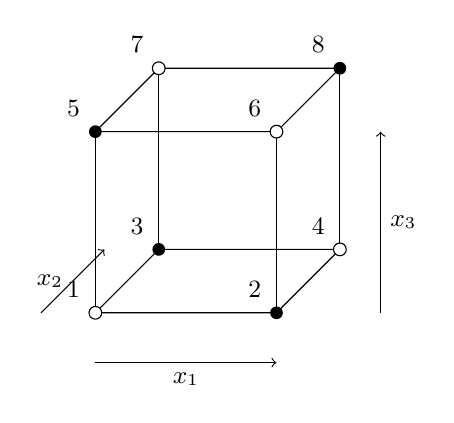
\begin{tikzpicture}[scale=1.15,every node/.style={font=\small}]
\coordinate (v1) at (0,0);\coordinate (v2) at (2,0);
\coordinate (v3) at (.7,.7);\coordinate (v4) at (2.7,.7);
\coordinate (v5) at (0,2);\coordinate (v6) at (2,2);
\coordinate (v7) at (.7,2.7);\coordinate (v8) at (2.7,2.7);
\draw (v1)--(v2)--(v4)--(v3)--cycle;
\draw (v5)--(v6)--(v8)--(v7)--cycle;
\draw (v1)--(v5) (v2)--(v6) (v3)--(v7) (v4)--(v8);
\foreach \i in {1,4,6,7}{\draw[fill=white] (v\i) circle (2pt);}
\foreach \i in {2,3,5,8}{\fill (v\i) circle (2pt);}
\foreach \i in {1,...,8}{\node[above left=2pt] at (v\i) {\i};}
\draw[->] (0,-.55)--node[below] {$x_1$}(2,-.55);
\draw[->] (3.15,0)--node[right] {$x_3$}(3.15,2);
\draw[->] (-.6,0)--node[left] {$x_2$}(.1,.7);
\end{tikzpicture}
\caption{The full three-factor cube in standard order. Filled vertices have
\(x_1x_2x_3=1\); open vertices have product \(-1\). The same partition
defines two half fractions or two blocks. This records the cube and
alternate-corner constructions of the selected NIST sections.}
\label{fig:p15-factorial-cube}
\end{figure}

\section{Run order, center points, and blocked factorials}
\label{sec:p15-factorial-execution}

The polishing example uses the following low, middle and high settings:
\[
\begin{array}{c|rrr}
 &-1&0&1\\\hline
\text{Speed}&16&20&24\\
\text{Feed}&0.001&0.003&0.005\\
\text{Depth setting}&0.010&0.015&0.020
\end{array}.
\]
Coding is \((u-u_0)/h\), with half-ranges \(4,0.002,0.005\),
respectively. The full replicated table is the eight standard-order rows
above followed by the same eight rows. The source's randomized order of
those sixteen labeled runs is
\[
 5,15,9,7,3,12,6,4,2,13,8,16,1,14,11,10.
\]
Its nineteen-run schedule inserts \((0,0,0)\) at positions 1, 9 and 19
and fills the other positions in that order. These specifications recover
every row of its Tables 3.5--3.9. Running the original standard order could
align the third factor's four-low/four-high pattern with day/night drift;
randomization and recording execution conditions address that risk.

\begin{hbtheorem}{thm:p15-factorial-centers-blocks}{proved=annex:p15.factorial.centers-blocks}{What centers and block columns identify}
For a three-factor full factorial split by \(b(x)=x_1x_2x_3\), block I
contains rows \(1,4,6,7\) and block II rows \(2,3,5,8\).
On these eight corner rows the block column equals the three-factor
interaction column. A model with
both a free block coefficient \(\gamma\) and \(\beta_{123}\) identifies
their sum, while the main and two-factor columns remain orthogonal to it.
If the center is then observed in both blocks, a common center response
with additive block effects gives a between-block center contrast
\(2\gamma\). Combining it with the corner contrast
\(2(\gamma+\beta_{123})\) separates \(\gamma\) and \(\beta_{123}\)
under that enlarged model.

In a quadratic response model
\(\beta_0+\sum_j\beta_jx_j+\sum_{i<j}\beta_{ij}x_ix_j
 +\sum_jq_jx_j^2\), the mean at the center minus the equally weighted
corner mean is \(-\sum_jq_j\). Corners and the common center do not
separate the individual \(q_j\), because their square columns coincide.
Adding center rows to the fraction \(x_3=x_1x_2\) likewise does not
separate \(\beta_3\) from \(\beta_{12}\).
\end{hbtheorem}

The corner-only block construction gives up a high-order comparison.
Interpreting its fitted block coefficient as a pure block effect requires
an assumption about the aliased interaction. Center points provide repeated
observations and a curvature or drift diagnostic under the corresponding
model; they do not identify every quadratic term or remove every alias.
Within-block replication and randomization retain their own assignment unit.

\section{Regular fractions, generators, and aliases}
\label{sec:p15-factorial-fractions}

\begin{hbdefinition}{def:p15-factorial-fraction}{A regular two-level fraction}
Represent a word by a subset \(S\subseteq\{1,\ldots,k\}\), with
column \(\chi_S\). Multiplication is symmetric difference:
\(\chi_S\chi_T=\chi_{S\mathbin{\triangle}T}\), and the empty word
is the intercept \(I\). A regular fraction is specified by \(p\)
independent word equations
\(\chi_{G_j}=s_j\), with \(s_j\in\{-1,1\}\).
Independence means that no nonempty product of the selected generator words
is the empty word.
Their products form a group \(\mathcal G\) of \(2^p\) words, with
assigned signs \(s(H)\). The full defining relation includes every
nonempty word in this group, not only the chosen generators. Positive
generator signs give the principal fraction.
\end{hbdefinition}

\begin{hbtheorem}{thm:p15-factorial-alias}{proved=annex:p15.factorial.alias}{Run count and the exact alias relation}
The regular fraction has \(2^{k-p}\) runs and
\[
 \frac1{2^{k-p}}\sum_{x\text{ in fraction}}\chi_S(x)\chi_T(x)
 =\begin{cases}s(S\mathbin{\triangle}T),&S\mathbin{\triangle}T\in\mathcal G,\\
 0,&\text{otherwise}.
 \end{cases}
\]
Columns in the same word coset are identical up to their stated signs;
columns from different cosets are orthogonal. For a full factorial mean
function \(\sum_T\beta_T\chi_T\), the normalized contrast on a fraction
has expectation
\[
 \mathbb E\!\left[\frac1{2^{k-p}}\sum_x\chi_S(x)Y_x\right]
   =\sum_{H\in\mathcal G}s(H)\beta_{S\mathbin{\triangle}H}.
\]
It estimates this alias sum without an assumption that the other terms vanish.
\end{hbtheorem}

\begin{hbdefinition}{def:p15-factorial-resolution}{Resolution and aberration}
The resolution is the smallest size of a nonempty word in the defining
relation. Its usual label is a Roman numeral. The word-length counts record
how many defining words have each size; comparisons of aberration examine
these counts from the shortest lengths upward. Such a comparison is about
an alias pattern, not evidence that the aliased physical effects are small.
A full factorial, whose defining group has no nonempty word, may be assigned
infinite resolution for these comparisons.
\end{hbdefinition}

\begin{hbcorollary}{thm:p15-factorial-resolution}{proved=annex:p15.factorial.resolution}{Resolution III, IV, and V}
At resolution III, distinct main effects are not aliased, but some main
effects are aliased with two-factor interactions. At resolution IV, main
effects are clear of all two-factor interactions, while some two-factor
interactions are mutually aliased. At resolution V, main effects and
two-factor interactions are clear of one another, but some two-factor
interactions are aliased with three-factor interactions. These statements
do not separate any effect from every possible higher-order interaction.
For resolution at least V, the intercept, all \(k\) main effects and all
\(\binom{k}{2}\) two-factor columns are linearly independent. Thus
\(N\geq1+k+\binom{k}{2}\). For eight factors this is \(N\geq37\);
a regular power-of-two fraction therefore needs at least sixty-four runs.
\end{hbcorollary}

A resolution-II design aliases some main effects with one another. It may
still estimate a specified sum or other row-space functional; it does not
supply their separate values without additional information.

\section{The half fraction and the cost of a sparsity assumption}
\label{sec:p15-factorial-half}

The following table gives the two-factor base, its product column, and both
three-factor half fractions. It retains the constructions of the source's
Tables 3.12--3.15:
\[
\begin{array}{c|rr|r|rr}
 &x_1&x_2&x_1x_2&x_3=+x_1x_2&x_3=-x_1x_2\\\hline
1&-1&-1&1&1&-1\\2&1&-1&-1&-1&1\\
3&-1&1&-1&-1&1\\4&1&1&1&1&-1
\end{array}.
\]
For the principal fraction, \(I=123\), and the complete alias classes are
\[
 I=123,\qquad 1=23,\qquad2=13,\qquad3=12.
\]
The last two analysis columns \(x_3,x_1x_2\) coincide. Replacing
\((\beta_3,\beta_{12})\) by
\((\beta_3+t,\beta_{12}-t)\) leaves every fitted response unchanged.
Only their sum is recovered. For the negative fraction the signs reverse:
\(I=-123\), \(1=-23\), \(2=-13\), \(3=-12\).

\begin{hbexample}{def:p15-factorial-nist-effects}{Full and fractional contrasts in the source data}
The source's standard-order responses are
\[
 (33,63,41,57,57,51,59,53).
\]
Its full factorial has intercept \(51.75\) and factorial effects in order
\((1,2,12,3,13,23,123)\) equal to
\[
 (8.5,1.5,-3.5,6.5,-14.5,0.5,3.5).
\]
On rows \(1,4,6,7\), the negative fraction, the three main-column
contrasts are \((8,16,10)\). They equal
\((8.5-0.5,\,1.5-(-14.5),\,6.5-(-3.5))\), precisely the predicted
alias differences. The corresponding principal-fraction contrasts are
\((9,-13,3)\). There is no conflict between these computations: the
fractions estimate different sums of full factorial effects.
\end{hbexample}

In the source's fifteen-run budget example, a twice-replicated full cube
already requires sixteen runs. A twice-replicated half fraction uses eight,
leaving seven for centers and contingencies. Its displayed thirteen-run
schedule is
\[
 000,\ +--,\ -+-,\ 000,\ +++,\ --+,\ 000,\ +--,
 \ --+,\ 000,\ +++,\ -+-,\ 000.
\]
Here the third coordinate is the product of the first two at the corners;
the center indicator is one exactly on the five \(000\) rows. This
specifies every row of Table 3.16. If interactions matter, an unreplicated
full cube plus centers may instead preserve the necessary effect separation.
Neither choice removes the need to justify its variance and mean model.

\section{Eight-factor designs and the source catalogue}
\label{sec:p15-factorial-eight}

For eight factors in thirty-two runs, the first source construction starts
with five freely varied columns and generates
\[
 6=345,\qquad7=1245,\qquad8=1235.
\]
Its full defining relation is
\[
 I=3456=12457=12358=12367=12468=3478=5678.
\]
Together with the standard-order formula in
\cref{def:p15-factorial-walsh}, these equations specify the complete
thirty-two-row design matrix. The resolution is IV. The aliased two-factor
groups are
\[
 34=56=78,\quad35=46,\quad36=45,\quad37=48,
 \quad38=47,\quad57=68,\quad58=67.
\]
These involve fifteen of the twenty-eight two-factor interactions.
The thirteen involving factor 1 or factor 2 are clear of other two-factor
interactions, though higher-order aliases remain.

The source's alternative \(6=12345,7=135,8=245\) has defining relation
\[
 I=123456=1357=2458=2467=1368=123478=5678.
\]
Its two-factor alias groups are
\[
\begin{gathered}
13=57=68,\quad15=37,\quad17=35,\quad24=58=67,\\
25=48,\quad28=45,\quad26=47,\quad27=46,\\
16=38,\quad18=36,\quad56=78.
\end{gathered}
\]
Exactly four two-factor interactions, \(12,14,23,34\), are clear of other
two-factor interactions. Thus twenty-four are aliased. The five length-four
words make this pattern less favorable than the first construction's three
length-four words under the stated short-word comparison.

A third displayed specification is \(6=123,7=124,8=2345\). It is a
relabeling of the first defining group by
\[
 (1,2,3,4,5,6,7,8)\longmapsto(5,8,1,2,3,6,4,7).
\]
The image of its three original generators spans the same word group,
so the alias structure is unchanged up to this factor permutation.

The following catalogue preserves all design specifications in the selected
2012 Table 3.17. An entry \((k,p;R;N)\) denotes \(2^{k-p}_R\), with
\(k\) factors, \(p\) independent generators, resolution label \(R\)
and \(N\) runs. It is a source catalogue, not a claim that a design's
resolution alone meets a particular scientific target.
\[
\begin{array}{rrrr|rrrr|rrrr}
k&p&R&N&k&p&R&N&k&p&R&N\\\hline
3&1&\mathrm{III}&4&4&1&\mathrm{IV}&8&5&1&\mathrm V&16\\
5&2&\mathrm{III}&8&6&1&\mathrm{VI}&32&6&2&\mathrm{IV}&16\\
6&3&\mathrm{III}&8&7&1&\mathrm{VII}&64&7&2&\mathrm{IV}&32\\
7&3&\mathrm{IV}&16&7&4&\mathrm{III}&8&8&1&\mathrm{VIII}&128\\
8&2&\mathrm V&64&8&3&\mathrm{IV}&32&8&4&\mathrm{IV}&16\\
9&2&\mathrm{VI}&128&9&3&\mathrm{IV}&64&9&4&\mathrm{IV}&32\\
9&5&\mathrm{III}&16&10&3&\mathrm V&128&10&4&\mathrm{IV}&64\\
10&5&\mathrm{IV}&32&10&6&\mathrm{III}&16&11&4&\mathrm V&128\\
11&5&\mathrm{IV}&64&11&6&\mathrm{IV}&32&11&7&\mathrm{III}&16\\
15&11&\mathrm{III}&16&31&26&\mathrm{III}&32&&&&
\end{array}
\]
The source also identifies a sixty-four-run resolution-V option for eight
factors and a forty-eight-run three-quarter alternative. The latter is
not a regular power-of-two fraction governed by the word-group formula.
Its separate construction and the linked Dataplot catalogue files are
external source referrals, not additional rows in the selected compiled
sections. For letter notation, factors 1 through 11 correspond to
\(A,B,C,D,E,F,G,H,J,K,L\); \(I\) denotes the intercept.
The sixteen-run, fifteen-factor and thirty-two-run, thirty-one-factor
entries are saturated for a main-effects model: even that restricted model
uses every observation-space dimension.

Screening designs trade run count against reliance on small-interaction
assumptions. Follow-up designs may add runs to separate important aliases
or add levels to study curvature. Different generators with the same run
count and resolution can protect different contrasts. A contrast should
therefore be checked against the actual defining relation or the row space,
not inferred from a resolution label alone.

\section{Assignment effects and mechanism claims}
\label{sec:p15-factorial-causal}

\begin{hbdefinition}{def:p15-factorial-assignment}{A finite assignment experiment}
Fix \(N\geq1\) recruited units, a nonempty finite set of treatment cells
\(\mathcal T\), and real potential responses \(Y_i(t)\).
Let \(Z_i\) be the randomized assigned
cell and \(\pi_i(t)=\Pr(Z_i=t)>0\). Stable treatment versions,
consistency and no relevant interference mean that the recorded outcome
for a retained unit is \(Y_i(Z_i)\). Randomness here is the known
assignment mechanism; it is separate from random sampling of a population.
For fixed weights \(w_t\), define
\(\tau=N^{-1}\sum_i\sum_tw_tY_i(t)\).
\end{hbdefinition}

\begin{hbtheorem}{thm:p15-factorial-assignment}{proved=annex:p15.factorial.assignment}{Which assignment contrast is unbiased?}
Under the preceding assignment model,
\[
 \widehat\tau=\frac1N\sum_i\sum_t
  \frac{w_t\mathbf1_{\{Z_i=t\}}Y_i(t)}{\pi_i(t)}
\]
is unbiased for \(\tau\). For a completely randomized design with fixed
positive cell sizes \(n_t\), it equals \(\sum_tw_t\overline Y_t\).
Its exact randomization variance is
\[
 \frac1{N^2}\sum_{i,t,j,u}
 \frac{w_tw_uY_i(t)Y_j(u)}{\pi_i(t)\pi_j(u)}
 \bigl(\pi_{ij}(t,u)-\pi_i(t)\pi_j(u)\bigr),
\]
where \(\pi_{ij}(t,u)=\Pr(Z_i=t,Z_j=u)\), also for \(i=j\).
This identity can involve unobserved potential responses; it is not itself
an observable variance estimator.
\end{hbtheorem}

For the P19 targets, use weights \((0,0,-1,1)\) for the aid-present
checking contrast and \((-1,1,-1,1)/2\) for its equal-weight average.
Blocked assignment uses its actual marginal and joint probabilities and
the desired block weights. Differential missing outcomes, incompatible
unit definitions or interference can break the displayed observation
model. Noncompliance does not change an assignment contrast into an effect
of receiving the instruction. Generalization beyond the recruited units
requires a sampling or transport argument.

\begin{hbtheorem}{thm:p15-factorial-mechanism}{proved=annex:p15.factorial.mechanism}{The factorial surface does not identify a psychological mechanism}
There exist two finite causal models with the same responses under every
assignment of checking \(A\) and aid \(B\), including the surface
\(4-4A-4B+6AB\), but different responses to intervening on a putative
reflection variable. Hence complete estimation of the factorial surface,
even without sampling error, does not identify that mechanism.
\end{hbtheorem}

The required additional evidence concerns the competing mechanisms:
process measurements with an explicit measurement model, interventions or
controls that separate them, and assumptions connecting those observations
to the causal equations. Statistical estimability, model-based uncertainty,
an effect of randomized assignment and a mechanism interpretation each have
their own premises. The distinction agrees with the intervention and
identification definitions in \cref{def:p16-causal-intervention,def:p16-causal-identification}.
